\documentclass{article}
\usepackage[utf8]{inputenc}
\usepackage[T1]{fontenc}
\usepackage[english]{babel}
\usepackage{enumitem}
\usepackage{amssymb}
\usepackage{color}
\usepackage[colorlinks,linkcolor=myorange, urlcolor=mygray, citecolor=mygreen, breaklinks, pagebackref]{hyperref}
\usepackage{graphicx}
\usepackage{caption}

\definecolor{mygray}{rgb}{0.7,0.7,0.7}
\definecolor{mygrey}{rgb}{0.5,0.5,0.5}
\definecolor{myorange}{rgb}{0.9,0.5,0}
\definecolor{mygreen}{rgb}{0.4,0.8,0}
\newenvironment{itemh}[0]{\begin{itemize}[label=$\heartsuit$, font=\color{mygray} \small]}{\end{itemize}}
\newenvironment{itemH}[0]{\begin{itemize}[label=$\heartsuit$, font=\color{mygray} \large]}{\end{itemize}}

\begin{document}
\title{Comparative Study about intelligent agents on RDF's graphs\\
	\textit{Bachelor Project in Semantic Web using bee and ant agents}}
\author{	Baudouin Duthoit\\
		Student number : 2540566
	\and
		Wouter Beek
	\and
		Stefan Schlobach
	}
\maketitle

\abstract{
	RDF is a standard of W3C to enable computer and human to understand data, to give them sense.
	That is the Semantic Web.
	Data is stored in triples formed of a subject and a predicate and an object.
	Those triples themselves are on different computers well spread all over the web.
	More and more people are using the Semantic Web and so the online data is increasing a lot
	making the reasoning over the graph really complex and the more complex it is,
	the more we need efficient agents to increase performances.
	Our goal is to create agents that performs that reasoning base on the ants behaviour
	and compare them to the bee agents we already have, created last year by Christophe Guéret.
	Those agents are coded in JavaScript and perform as a Web application that any client can use,
	an example of the pre-existing project can be found here \url{http://wouterblog.com/} .
}

\newpage

\tableofcontents

\newpage

\section{Introduction}
	%Introduction to RDF / Semantic Web
	\paragraph{} % Global presentation of RDF : The semantic web \& RDF
		Since its creation, the web see its data increasing exponentially.
		Those data are often unstructured and only human readable.
		Facing those two problems, scientists invented the semantic web to aggregate data
		and make it easy to access for humans and computers.\cite{Grigoris12}
		Those meta-data are structured in triples that are stored online in a lot of different places in RDF
		(Resource Description Framework).
		Each triple is made of a subject, a predicate and an object.
		We can see it as 2 nodes and an arc (predicate) from the subject to the object, thus we get an oriented graph.
		Also, there are several ways to store this data online.
	\paragraph{}	% Data format
		The most common one is to put the data on a database and query it via SPARQL,
		which is language that look like SQL but for RDF.
		Then we can send a query and get back some results that are in that database.
		As for SQL, SPARQL could built some complicated queries.
		The other common way of getting data is directly get files containing RDF in it (turtle, rdf, n3).
		The last one is with deferenced data which is a mix of the two :
		it ask the server for data about a resource and get a file containing the data.
	\paragraph{}	%Introduction to other work
		Last year, another bachelor student worked on a similar project.
		His goal was to get back information from a search using agents acting like bees (in JavaScript) \cite{Kroes13,Kroes13-2}.
		We used his code as inspiration for our own bees agents (that are programmed in prolog).
		That work was based on a paper \cite{Gueret10} about Swarm computing.
		The project repository is on GitHub\footnote{\url{https://github.com/wouterbeek/DataHives}},
		it is mostly using SWI-Prolog\footnote{Official web-site: \url{http://swi-prolog.org/}} language.
	%	\paragraph{}	%Introduction to DataHives subsection
	%	\project{Hypothesis}
		\begin{center}
			\textit{
			\textbf{Hypothesis :} In this project, we will compare the graphs induced by the bee walk,
				to the one obtain by the random agents and also the one induced by the ant walk.
				We expect to have a high number of cluster of high betweenness centrality on the bee graph,
				and a pagerank-like graph for the random agents.
				The ants have a few components and a high connected one}
		\end{center}

	%	\subsection{Evaluation}
		\paragraph{Evaluation:}
			We will verify the hypothesis via different criteria.
			We'll make them work for a certain time and then compute the betweenness centrality and the clustering coefficient.
			We will also variate the number of agents to see if there are some big variations or not (saturation ?).
			Those two methods will be used to compare 3 kind of agents:
		\begin{itemh}
			\item Random (basic)
			\item Bee (translated from JavaScript)
			\item Ant (Implemented from scratch)
		\end{itemh}

\newpage
\section{Approach}
	\paragraph{}
		Our work on the agents is based on this book \cite{Engelbrecht05}.
		All the agents are implemented in the same way.
		They follow a cycle of events and repeat that cycle.
		The cycle to follow is :
	\begin{center}
		Navigate / Act / Communicate / Evaluate
	\end{center}
	\paragraph{}
		Navigation is the function that decide \textbf{where} the agent should go, depending on where it is already.
		In facts, this predicate pick a proposition between all the possibilities,
		those possibilities are all nodes that are neighbours to the one we are on.
		The graph containing all the neighbours is called the ego-graph of the chosen node,
		we assume it contains all the incoming and out going neighbours.
		Unfortunately, those nodes could be literals and then we could get stuck on it because literals are linked to nothing.
		To avoid that, we have a backtrack function that keeps in mind the last position we were on.
	\paragraph{}
		Acting is where the agent do what it is meant for when it is on his own.
		In a clearer way it means that in this step the agent should work on the nodes it is on.
		This step is a selfish one where the other agents don't matter at all.
		The main action is only the deductive action of entailment.
		The rules for that can be found on the W3C web page\footnote{\url{http://www.w3.org/TR/2014/REC-rdf11-mt-20140225/\#rdfs-entailment}}.
		We apply all of them to get some more information.
		Because all agents will have the same action, we decide to describe it here.
	\paragraph{}
		Communication is the main point of those agents.
		We try different kind of communication to see whether one is more efficient than the other
		and then compare the different kind of agents.
	\paragraph{}
		The evaluation part decides whether an agent deserve to continue his job or not.
		If it is judge inefficient then we throw it away using the exit function given at the creation of the agent.
		It's here where the fitness function should act.
	\subsection{Random Agent}
		\subsubsection{Navigate}
			\paragraph{}
			The random agent is implemented to go randomly.
			It is initialized on a set of available URI where to begin.
			Then it goes, following "links".
			Those links are the predicates between 2 nodes of the Linked Open Data (LOD).
		\subsubsection{Communicate}
			\paragraph{}
			The communication is not implemented to stick a really basic agent attitude that will serve as reference for efficiency.
		\subsubsection{Evaluate}
			\paragraph{}
			The evaluation function is not set for this kind of agent that keep going whatever happens.
		\subsubsection{At exit}
			\paragraph{}
			This predicate is not used because it is really bound to the evaluation that we discarded.
	\subsection{Ant Agent}
		\subsubsection{Navigate}
			\paragraph{}
			The ant navigation is based on randomness but a weighted one.
			Like an ordinary ant, our agent has to pick a path, depending on the pheromones left on it.
			On the virtual web of the LOD, the pheromones are coefficient left on edges from one node to the other.
			If another ant went here before, the path get more value.			
		\subsubsection{Communicate}
			\paragraph{}
			As said above, an ant leave pheromones in an intelligent way.
			The insect is looking for food (= information) outside (= on the LOD).
			When it has found something, it goes back to the anthill and leave pheromones on its way back as well.
			The main idea here is to up value a path which leads to food and devalue one that leads nowhere (ie dead-end path).
			To represent this in a virtual way here was our main ideas $c \in \mathbb{R}$:
			\begin{itemh}
				\item Devalue dead end path, using SPARQL queries to go back and degrade the weight of the path of $c$
				\item Adding $c$ to all the travelled path for each information deduced
				\item Adding the agent's current fitness to the current edge
			\end{itemh}
			\paragraph{}
				All those ideas needs to be evaluated and tried to see which one is the more efficient and if we could cross them.
		\subsubsection{Evaluate}
			\paragraph{}
			The evaluation is where the fitness function enter in the game.
			For the ants, the fitness function is quantitative,
			counting the number of triples discovered via deduction and dividing it by the number of steps taken.
			If that number is bigger than 0.5, the agent can live, otherwise it dies launching the exit function.
		\subsubsection{At exit}
			\paragraph{}
			When the time comes for an agent to kill himself, it is decided that it must launch another agent to replace him.
			And so, the agent launch another agent that will work to get more information that the previous one if possible.
	\subsection{Bee Agent}
		\subsubsection{Navigate}
			\paragraph{}
			A bee navigates randomly, whatever her role is.
			It goes to a random place and then another random place, and keep going in doing this.
			The scouts are wandering around to try to find information.
			When one succeed, it tells some others (called forager) to come and grab the "pollen" it has found.
		\subsubsection{Communicate}
			\paragraph{}
			Here the communication is really simple.
			It directly contact the other agent to tell them something : the information is not sustainable, it is not stored somewhere.
			The information send is used instantly (it makes it more easy to set up).
		\subsubsection{Evaluate}
			\paragraph{}
			The evaluation is based on the same criteria of the one for the ants but here it trigger an action.
			If the fitness is big enough we send some foragers helping the scout, but if it is too low ... the agent get killed.
		\subsubsection{At exit}
			\paragraph{}
			At the end of the thread we also ask for another agent to replace the bad one and keep sustainability in getting information.

\section{Implementation}
	\subsection{Developping tools}
		\subsubsection{Prolog}
			
	\subsection{Debug tool}
		\paragraph{}
			This section will present to you what features already implemented in the project are in use.
			What we have access in this interface to the graph the agents have been crawling.
			It is a way of visualize the graph that as been created by the agents.
			It has also been used as a debug tool: if the graph contained only one node with one edge where the agent passed 200 times,
			that means that there is something fishy about the navigation strategy.
			Another good example was with the bee algorithm, where a lot of nodes where alone, with no neighbours.
			In that case, it meant that the communication or the evaluation was wrong (either calling forager or the fitness were bad).
			\begin{figure}[!h]
				\hspace{-2cm}
				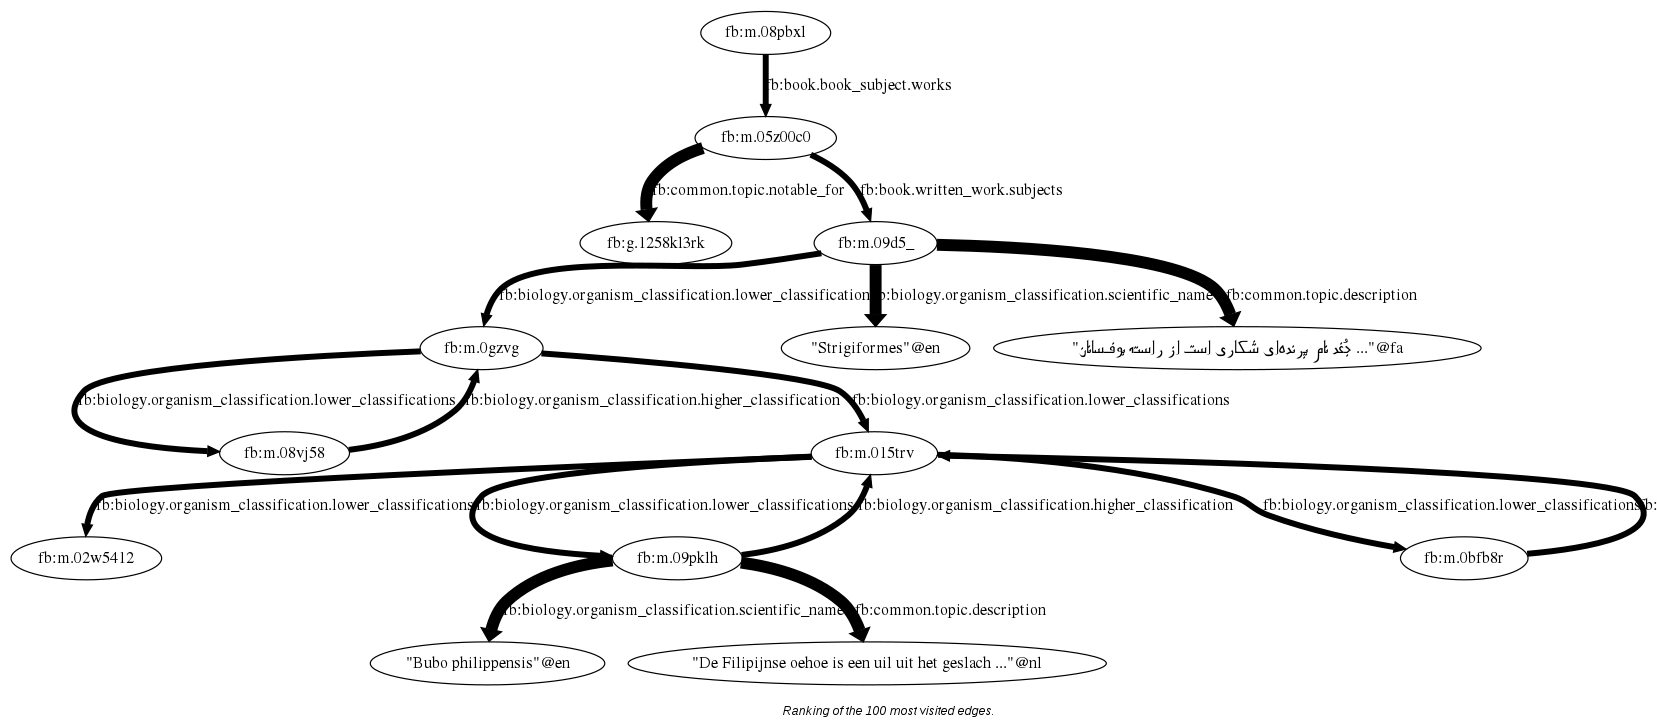
\includegraphics[width=1.4\textwidth]{../dh_graph}
				\captionof{figure}{Sketch of the graph}
			\end{figure}
			\paragraph{}
				This Web interface also enable show a table containing all the agents working at the moment on the graph with their status.
				If one of the agent crash, it shows up and the reason why.

\section{Evaluation}
	\subsection{Quantitative Evaluation}
		\paragraph{}
			First, we want to compare the agents over the number of deductions over the time they are running.
			It is something simple to count and objective, but it may be not relevant (if we look at the semantic part).
			To be more accurate, we have used 100 agents of each category, and run them for a certain time.
			Of course, it is running on the same machine to have the same environment as much as possible.
		\begin{center}
			\textit{Place for a future graph, comparing agents x = time, y = deductions}
		\end{center}
		\paragraph{}
			Description of the graph and deductions
	\subsection{Graph figures comparison}
		\paragraph{}
			We formulate in the hypothesis that the crawled graph must differ between every kind of agents.
			To prove this, we have been using Gephi
			\footnote{Here is the software website \url{https://gephi.github.io/}} to dig out some figures of our graphs.
			The more representation figures were the betweenness centrality and the clustering coefficient.
			The work on the graph is based on the content of the class "Networks ans graphs" followed this year,
			which was referenced on this book \cite{Steen10}.
		\paragraph{}
			For bees, we have a pretty high clustering coefficient of $0,026$ and the betweenness centrality is (on average) quite high.
			The betweenness centrality is a number that calculate for each node how many shortest path go through it.
			The highest this number is, the more important the node is.
			With bees, we expect to find a lot of nodes with a high betweenness centrality because for each node where a bee arrives on,
			there are $N$ potential foragers send from that node.
			Also, the clustering coefficient that describe how bounded are the nodes.
			With the bees, for the same reason that the one cited above,
			nodes are really close one from each other and are more likely to create a cluster
			(clusters are "natural" but relatively homogeneous groupings that are evident in a statistical population)
		\begin{figure}[!h]
			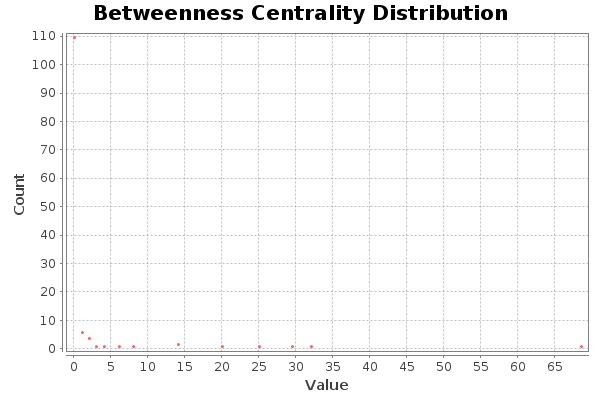
\includegraphics[width=1\textwidth]{dh_betweenness_centrality_bees}
			\captionof{figure}{Betweenness centrality figures for bees}
		\end{figure}
		\paragraph{}
			For random agents, the clustering coefficient is of $0$ and the betweenness centrality follow a classical curve.
			We can conclude that the graph does not have clear clusters.
			That was expected from the random graph, because the agents are just walking around.
			The expected behaviour is to find them on the more important nodes, have a Page-rank like behaviour.
		\begin{figure}[!h]
			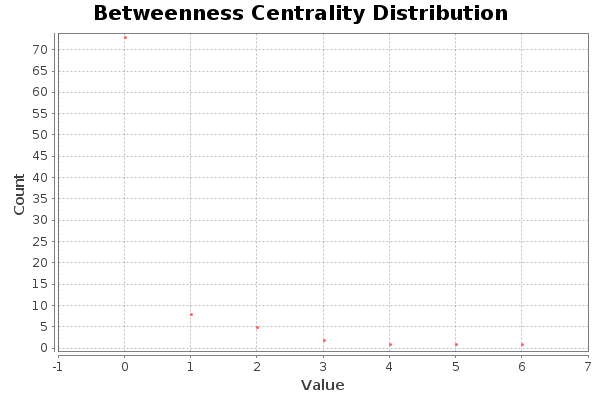
\includegraphics[width=1\textwidth]{dh_betweenness_centrality_random}
			\captionof{figure}{Betweenness centrality figures for random agents}
		\end{figure}
		
\section{Reflection}
	\subsection{Dead end paths}
		\paragraph{}
			The LOD is a big graph on which it is really easy to get lost.
			Especially in some dead end path, because the graph is oriented and going back is not easy.
			We have a backtrack function in case of which we would have arrived on a literal (special case),
			But this backtrack function is only limited to go one step backward.
			Storing the whole path would be memory inefficient.
		\paragraph{}
			To solve this, we start an action when an agent detect when it is in a dead end path (when it can't go anywhere).
			This specific action is quite simple, it start from the node where the agent got stuck and devalue the path to it.
			To know the path, we just crawl the cache starting from the "blocking node"
			and see if there is other possibilities that the one we come from.
			If yes, it means that the node we just arrived on is the end of the dead end path.
			If no, we just repeat the previous step to find that node which show the end of the path.
			Also, we kill the agent and create a new one instead that will crawl from another place.
	\subsection{Denied access}
		\paragraph{}
			The LOD contains some restricted area we the agents cannot go.
			When an agent meet such a place, it just go backward of one step.
			Sometimes, it is also because the server where we try to grab information from is down.
			Some of them, like dbpedia have a live version of it which is sometime replacing the other one,
			so we just try all different access point we knows to get data from.
	\subsection{Difficult tests}
		\paragraph{}
			At the beginning, the agents used to go really often in dead en alley
			or find information that is not in the right format and crashed.
			That made the testing quite complicated, because the data we got from those agent was too diverse to be relevant.
			The agents were to often far apart from each other (and the communication was quite useless then).
	\subsection{Keep as minimum the communication between threads}
		\paragraph{}
			Even if we want the agents to communicate with each other, it is better if their communication remain light,
			otherwise, they spend too much time waiting for each other and the efficiency becomes bad.
			For example, the system we work on don't have a kind of mother-ship that give orders.
			Each agent is working on his own and has is own independent functions.
		\paragraph{}
			A necessary communication that has been establish between threads is a message system to get information about the thread,
			like the number of steps taken.

\newpage
\section{Conclusion}
	\subsection{Results}
		\paragraph{}
			???
	\subsection{Thanks}
		\paragraph{}
			I would like to thanks the VU university from Amsterdam to makes me able to study here for this year.
			I also want to thanks Stefan for accepting me to do my Bachelor thesis with him
			and I especially thanks Wouter for his help during all this project.

\newpage
\bibliographystyle{plain}
\bibliography{bibliography}
\addcontentsline{toc}{section}{Bibliography}
\end{document}
